\subsection{Brain Tumor Classification (MRI)} \label{chap:Brain-Tumor}
Hirntumoren sind abnorme Zellwucherungen im Gehirn, die gutartig oder bösartig sein können. Diese Tumoren können entweder direkt im Gehirn entstehen oder als Metastasen von anderen Krebsarten in das Gehirn gelangen. Die Symptome variieren je nach Tumorart, -grösse und -lokalisation und umfassen häufig Kopfschmerzen, Übelkeit, Sehstörungen, Krampfanfälle und kognitive Beeinträchtigungen. Aufgrund ihrer Komplexität und der sensiblen Lage im zentralen Nervensystem stellen Hirntumoren eine erhebliche Herausforderung für die medizinische Diagnostik und Behandlung dar. Sie haben oft weitreichende Auswirkungen auf die Lebensqualität der Betroffenen.

Der \textbf{Brain Tumor Classification (\acrshort{mri})-Datensatz} \cite{bhuvaji_brain_2020} umfasst 3'260 bereinigte und \gls{augmentiert}e, T1-gewichtete, kontrastverstärkte \acrshort{mri}-Bilder zur Identifikation und Klassifikation von Hirntumoren.

Die in Abbildungen \ref{fig:brain-beispiele-klasse0} und \ref{fig:brain-beispiele-klasse1} gezeigten \acrshort{mri}-Bilder illustrieren Beispiele von Gehirnscans in Sagittal-, Frontal- und Transversalebenen des Kopfes, die zur Klassifikation von Hirntumoren verwendet werden. Positive Fälle sind mit der Klasse 1 und negative Fälle mit der Klasse 0 gekennzeichnet. Eine detaillierte Beschreibung der Klassenzusammenfassung findet sich in Kapitel \ref{chap:brain-datapartition}.

\begin{figure}[H]
    \centering
    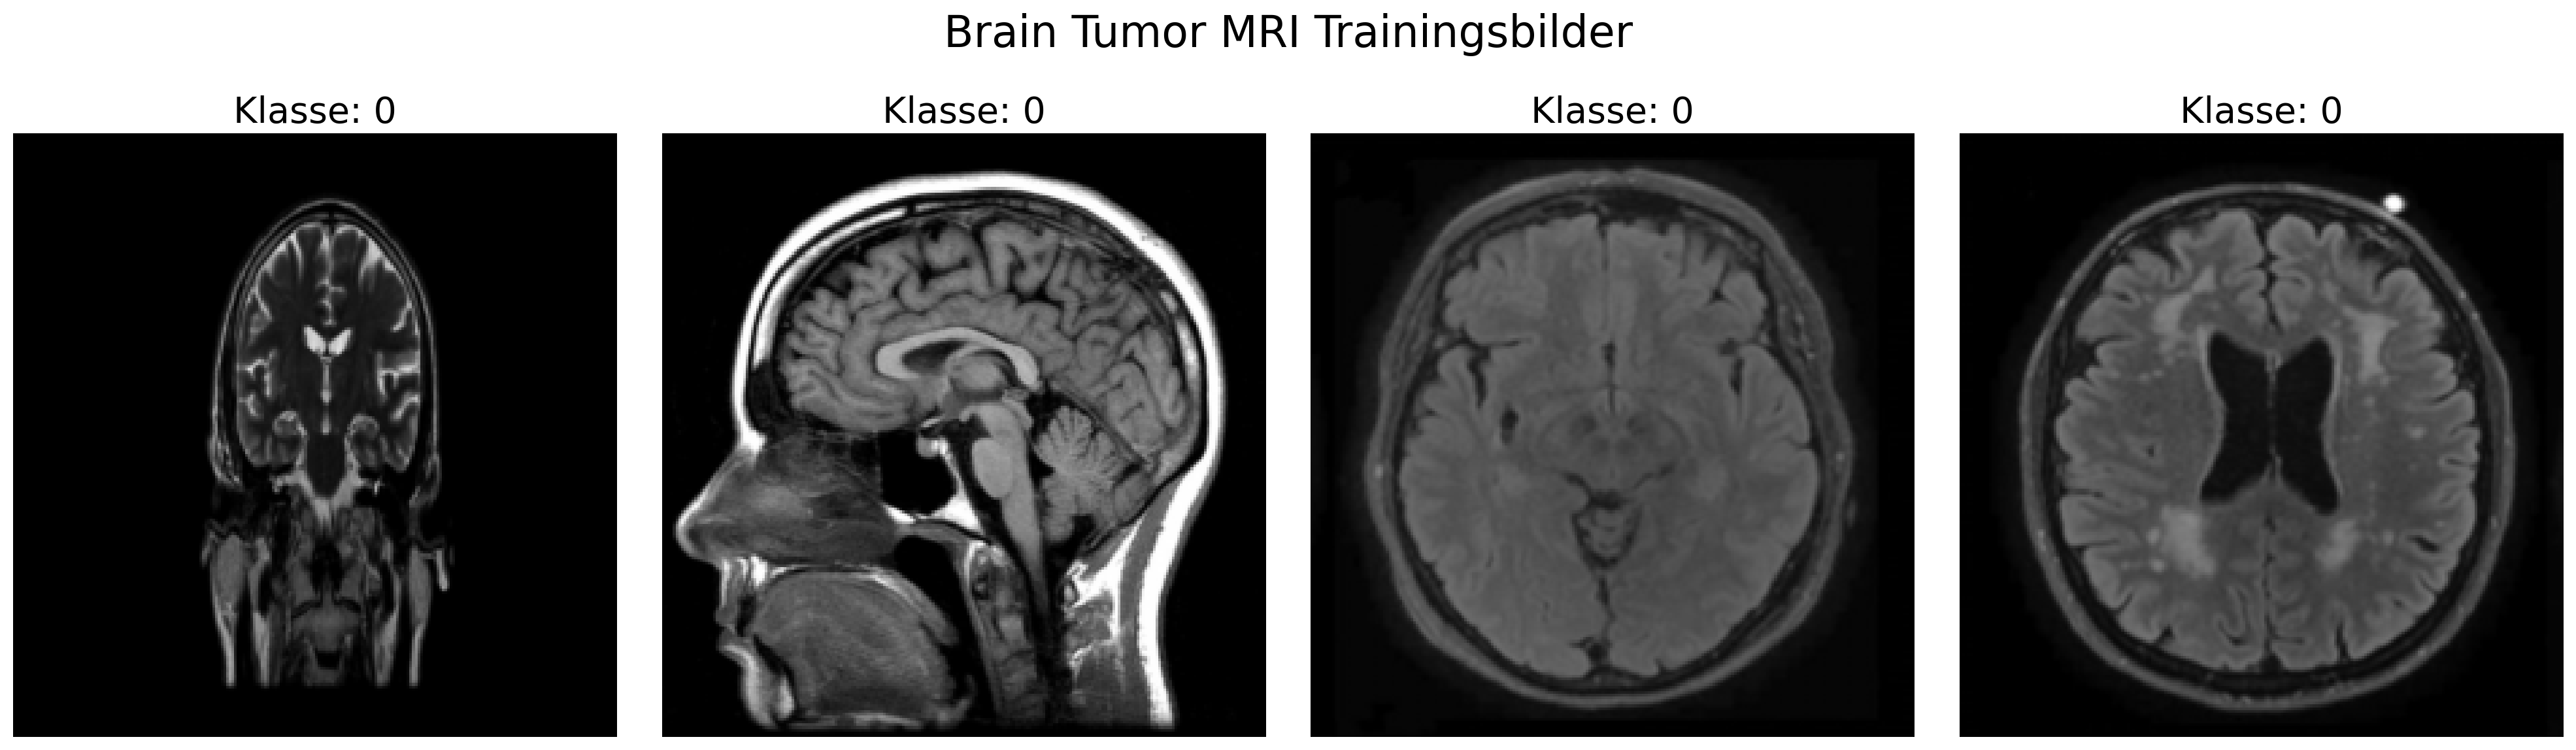
\includegraphics[width=\linewidth]{01-images/03-data/brain-klasse0.png}
    \caption{Beispiele von Patienten ohne Hirntumor Befund}
    \label{fig:brain-beispiele-klasse0}
\end{figure}

\begin{figure}[H]
    \centering
    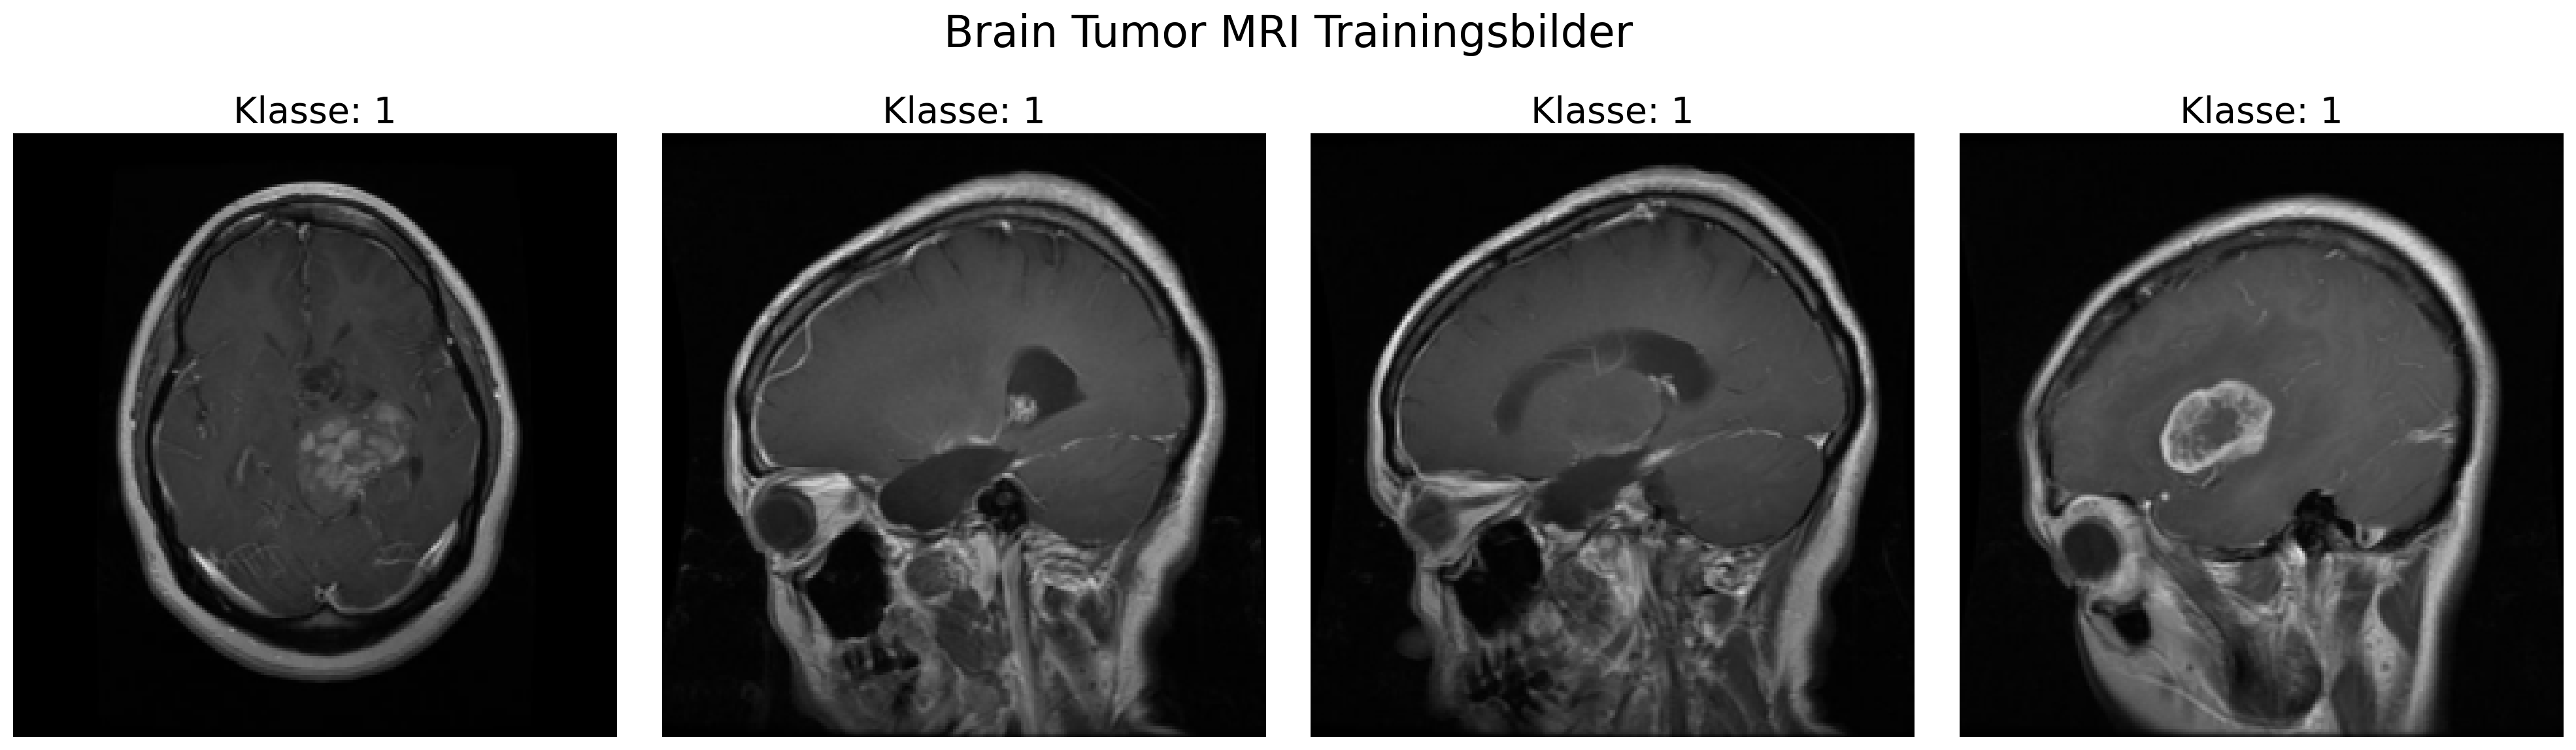
\includegraphics[width=\linewidth]{01-images/03-data/brain-klasse1.png}
    \caption{Beispiele von Patienten mit einem Hirntumor Befund}
    \label{fig:brain-beispiele-klasse1}
\end{figure}

\newpage

\subsubsection{Hirntumorarten} \label{chap:brain-hirnarten-datensatz}
Der Datensatz für Hirntumoren umfasst vier Klassen. Drei davon sind Fälle, in denen Hirntumoren vorhanden sind und eine Klasse enthält keine Hirntumoren. Die drei Klassen mit Hirntumoren sind Pituitary, Glioma, Meningioma.

\paragraph{Pituitary} \label{chap:brain-pituitary}
Pituitary Tumoren, auch als Hypophysenadenome bekannt, sind gutartige Tumoren der Hypophyse, einer kleinen Drüse im Gehirn, die wichtige Hormone produziert. Obwohl sie meist nicht bösartig sind, können sie aufgrund ihrer Lage und Hormonproduktion erhebliche gesundheitliche Probleme verursachen. Zu den Symptomen zählen häufig Kopfschmerzen, Sehstörungen und hormonelle Ungleichgewichte. Die Behandlung erfolgt in der Regel durch eine Operation und, in einigen Fällen, durch medikamentöse Therapie oder Strahlentherapie.

\paragraph{Glioma} \label{chap:brain-gliome}
Glioma bilden eine Gruppe von Hirntumoren, die im Glia-Gewebe des Nervensystems entstehen. Sie stellen die häufigsten primären Hirntumoren bei Erwachsenen dar und werden nach ihren Ursprungszellen in Astrozytome, Oligodendrogliome und Ependymome unterteilt. Die Symptome variieren je nach Lage und Grösse des Tumors und umfassen häufig Kopfschmerzen, Anfälle und neurologische Defizite. Die Behandlung erfolgt meist durch eine Kombination aus Operation, Strahlentherapie und Chemotherapie.

\paragraph{Meningioma} \label{chap:brain-meningioma}
Meningioma sind in der Regel gutartige Tumoren, die von den Meningen ausgehen, welche das Gehirn und Rückenmark umhüllen. Obwohl sie langsam wachsen, können sie durch Druck auf umliegendes Gewebe diverse Symptome verursachen, darunter Kopfschmerzen, Krampfanfälle und neurologische Ausfälle. Die Behandlung hängt von Grösse und Lage des Tumors ab und kann chirurgische Entfernung, Strahlentherapie oder in einigen Fällen auch eine abwartende Beobachtung umfassen. 

\newpage

\subsubsection{Datenpartitionierung} \label{chap:brain-datapartition}
Der Datensatz enthält ursprünglich nur einen Trainings- und Testdatensatz. Die Datenverteilung umfasste 87,9\% Trainings- und 12,1\% Testbilder. Da ein Validierungsdatensatz fehlt, wurde der ursprüngliche Trainingsdatensatz mittels stratifizierten Samplings in einen neuen Trainings- und einen Validierungsdatensatz aufgeteilt.  Der Datensatz umfasst drei Tumorklassen und eine Nicht-Tumorklasse. Die Verteilung der Klassen ist in Tabelle \ref{tab:brain-orginale-klassenverteilung} dargestellt. Diese zeigt, dass Tumorbilder deutlich häufiger vertreten sind als Nicht-Tumorbilder. Da die Modelle dieser Thesis auf binären Klassifikationsmodellen basieren, werden die drei Hirntumorklassen Pituitary, Glioma und Meningioma zu einer positiven Klasse zusammengefasst, während die Nicht-Tumorklasse als negative Klasse definiert wird. Dies wird in Tabelle \ref{tab:brain-binaere-klassenverteilung} dargestellt.

\begin{table}[H]
    \centering
    \begin{tabular}{@{}ccccc@{}}
        \toprule
         Partition & \multicolumn{4}{c}{Klassenverteilung}              \\ 
        \cmidrule(l){2-5}
                    & Pituitary & Glioma & Meningioma & kein Tumor      \\ 
        \midrule 
        Train      & 662 & 661 & 658 & 317                              \\
        Validation & 165 & 165 & 164 & 78                               \\
        Test       & 74  & 100 & 115 & 105                              \\ 
        \bottomrule
    \end{tabular}
    \caption{Ursprüngliche Klassenverteilung von Hirntumoren}
    \label{tab:brain-orginale-klassenverteilung}
\end{table}

Die Tabelle \ref{tab:brain-binaere-klassenverteilung} zeigt die Anzahl der Bilder in absoluter und relativer Häufigkeit sowie die Klassenverteilung von positiven und negativen Tumorbildern für jede Datenpartition.

\begin{table}[H]
    \centering
    \begin{tabular}{@{}cccccc@{}}
        \toprule
        Partition & \multicolumn{2}{c}{Anzahl Bilder} & \multicolumn{2}{c}{Klassenverteilung} & Positiv-Verhältnis\\ 
        \cmidrule(lr){2-3} \cmidrule(lr){4-5} 
                   & Absolut & Relativ & Positiv & Negativ  \\ 
        \midrule
        Train      & 2298 & 0.704 & 1981 & 317 & 0.862      \\
        Validation & 572  & 0.175 & 494  & 78  & 0.864      \\
        Test       & 394  & 0.121 & 289  & 105 & 0.736      \\ 
        \bottomrule
    \end{tabular}
    \caption{Datenpartitionierung vom Hirntumoren}
    \label{tab:brain-binaere-klassenverteilung}
\end{table}

\newpage

\subsubsection{Datenexploration} \label{chap:brain-eda}
Die Histogramme in den Abbildungen \ref{fig:brain-klasse0-hist} und \ref{fig:brain-klasse1-hist} zeigen die Pixelverteilung der \acrshort{mri}-Bilder von Patienten mit positiven und negativen Befunden aus Abbildung \ref{fig:brain-beispiele-klasse0} und \ref{fig:brain-beispiele-klasse1}. Jedes Histogramm stellt die Intensitätsverteilung der Pixelwerte in den jeweiligen Aufnahmen dar. Auf der x-Achse jedes Histogramms wird die Grauwertintensität von 0 bis 255 dargestellt, während die y-Achse die Anzahl der Pixel anzeigt. 

\begin{figure}[H]
    \centering
    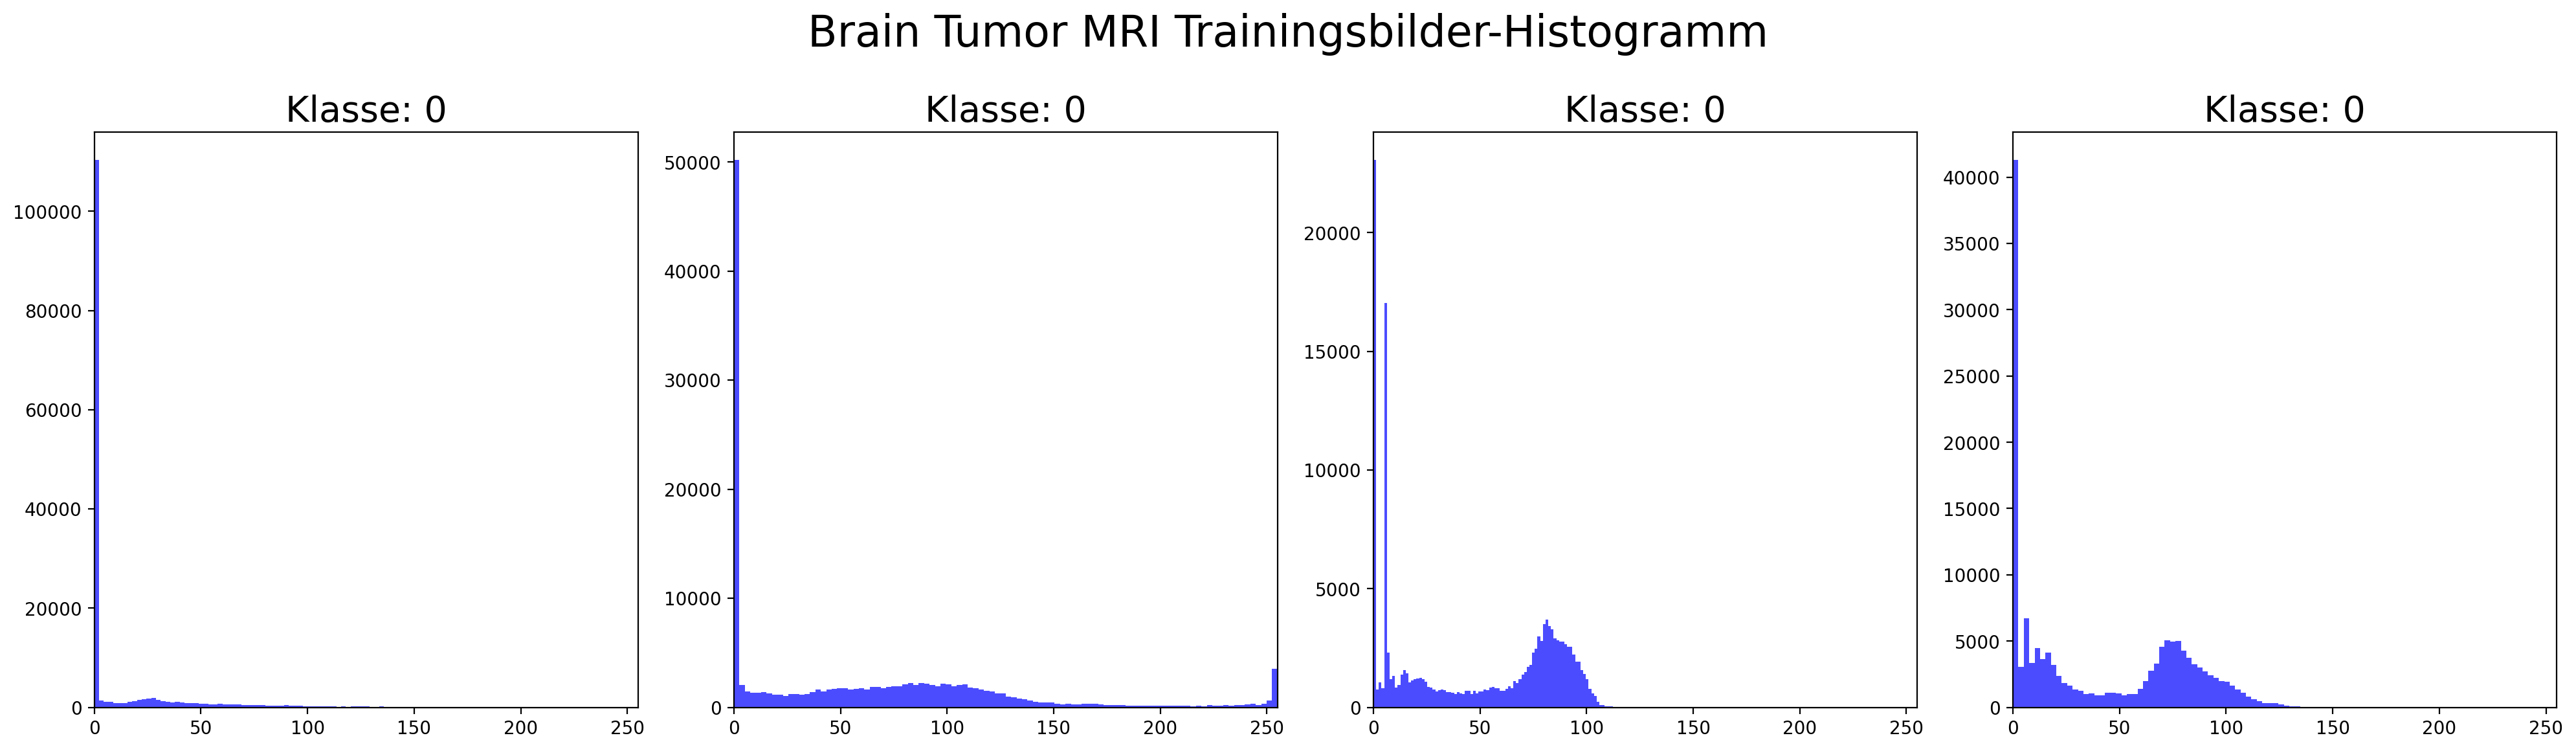
\includegraphics[width=\linewidth]{01-images/03-data/brain-klasse0-hist.png}
    \caption{Histogramm der Pixelverteilung von den Bildern aus Abbildung \ref{fig:brain-beispiele-klasse0} mit einer Bin-Grösse von 100}
    \label{fig:brain-klasse0-hist}
\end{figure}

\begin{figure}[H]
    \centering
    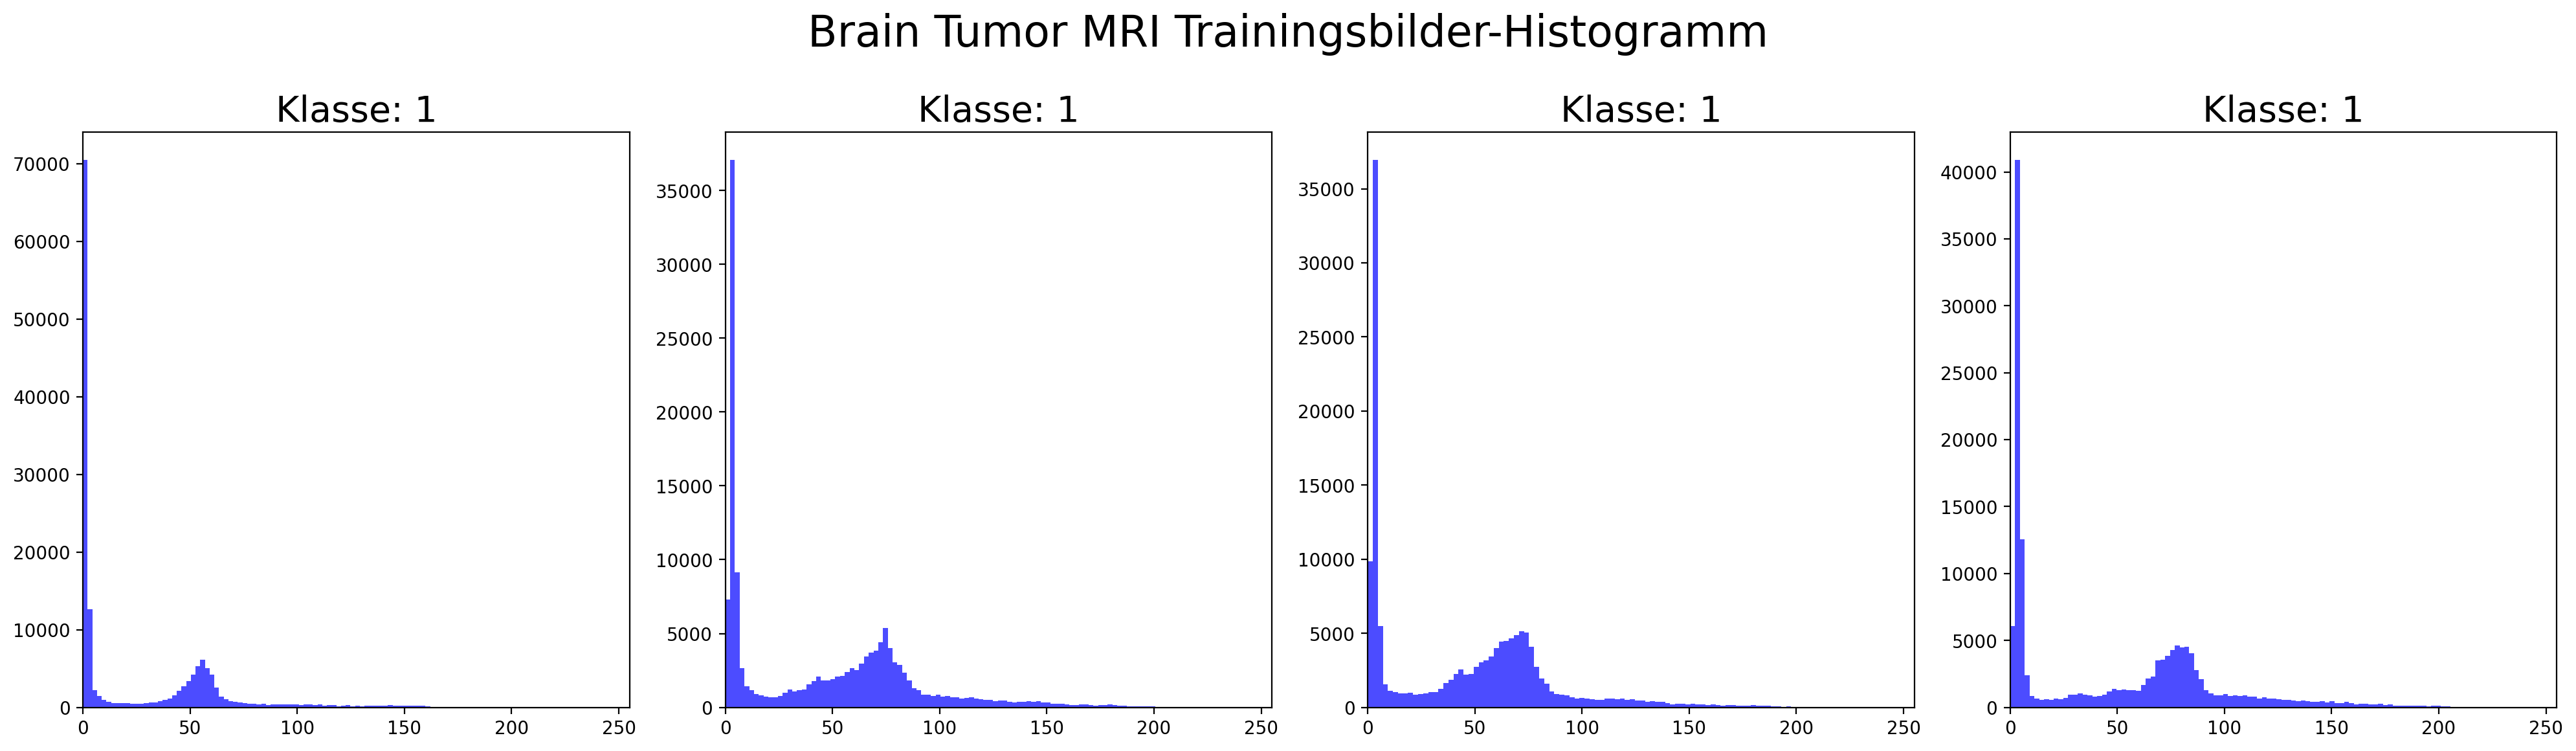
\includegraphics[width=\linewidth]{01-images/03-data/brain-klasse1-hist.png}
    \caption{Histogramm der Pixelverteilung von den Bildern aus Abbildung \ref{fig:brain-beispiele-klasse1} mit einer Bin-Grösse von 100}
    \label{fig:brain-klasse1-hist}
\end{figure}

Niedrige Pixelwerte in einem Bild weisen auf viele dunkle Bereiche hin. Dies deutet darauf, dass es sich um den Hintergrund der \acrshort{mri}-Bilder handelt, der einen Grossteil der Information enthält, aber keine relevanten Details.

\subsubsection{Datenverteilung} \label{chap:brain-datenverteilung}
Wie in Kapitel \ref{chap:COVID19-datenverteilung} beschrieben, stellte sich auch beim \acrshort{mri}-Datensatz das Problem der Performance auf den Testmetriken. Deswegen wird auch hier eine umfassende explorative Analyse der Trainings-, Validierungs- und Testdaten durchgeführt.

\newpage

\paragraph{Pixelverteilung} \label{chap:brain-pixelverteilung}
Das Vorgehen, das in Kapitel \ref{chap:COVID19-pixelverteilung} beschrieben wird, wird ebenfalls für die Partitionierung des Hirntumor-Datensatzes genutzt. Abbildung \ref{fig:brain-datapartition-pixelverteilung-histo} zeigt die Histogramme der Pixelwerte für jede Datenpartition.

\begin{figure}[H]
    \centering
    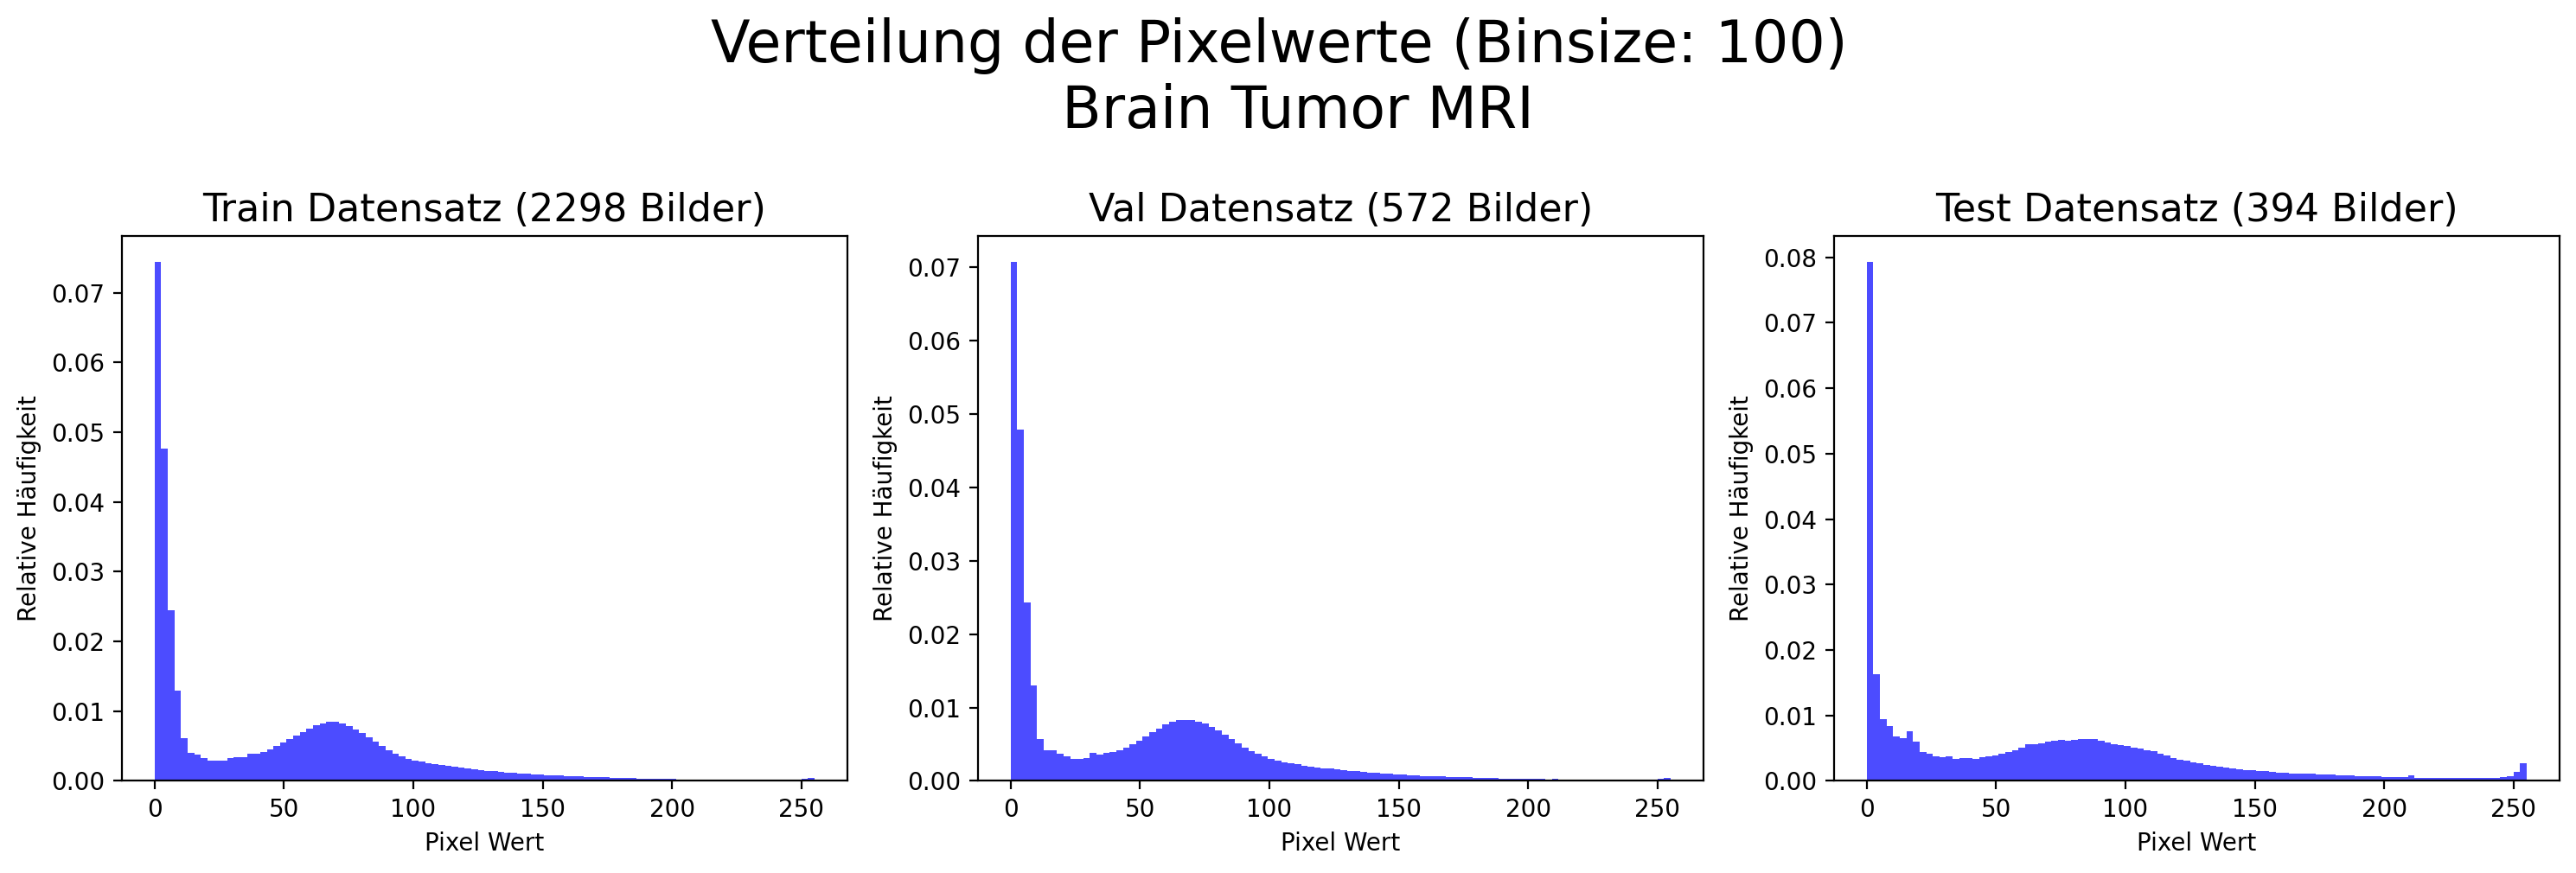
\includegraphics[width=\linewidth]{01-images/03-data/brain-Pixelverteilung-Partitionen.png}
    \caption{Histogramme der Pixelverteilung von jeder Datenpartition im Hirntumor Datensatz}
    \label{fig:brain-datapartition-pixelverteilung-histo}
\end{figure}

Die Pixelwertverteilung des Hirntumor-Datensatzes ähnelt dem Muster in Abbildung \ref{fig:covid-datapartition-pixelverteilung-histo}, weist jedoch einige Besonderheiten auf. Der charakteristische Buckel erscheint hier bei einem Pixelwert von etwa 80, wobei Trainings- und Validierungspartitionen ein nahezu identisches Verteilungsmuster zeigen. In der Testpartition ist der Buckel weniger ausgeprägt. Zudem weist die Testpartition einen markanten Anstieg ab einem Pixelwert von 250 auf, der in einem Ausschlag am Ende des Histogramms resultiert. Diese Abweichungen in der Testpartition deuten möglicherweise darauf hin, dass sie aus einer anderen Verteilung stammt als die Trainings- und Validierungspartition.

\paragraph{Pixelmittelwerte} \label{chap:Differenzenbilder-TestProblemEda2-mri}
Auch bei den Pixelmittelwerten erfolgt das Vorgehen analog zu dem in Kapitel \ref{chap:COVID19-pixelmittelwert} beschriebenen Verfahren.

\begin{figure}[H]
    \centering
    \begin{subfigure}[b]{0.49\linewidth}
        \centering
        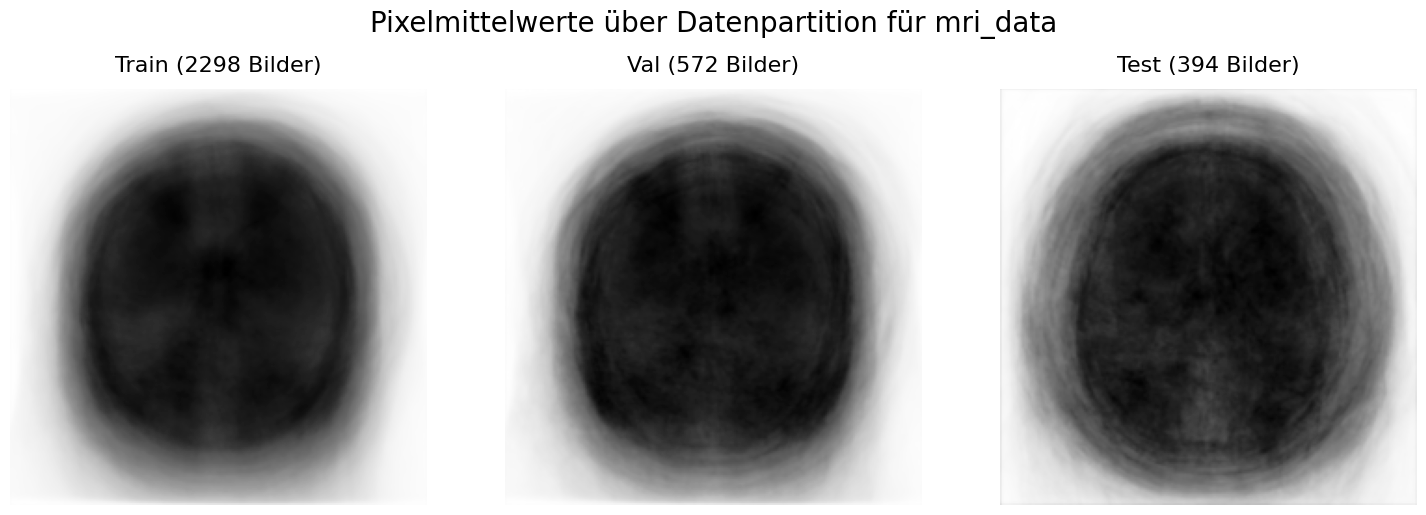
\includegraphics[width=\linewidth]{01-images/03-data/brain-pixelmittelwerte.png}
        \caption{Visuelle Darstellung der Pixelmittelwerte von aller Hirntumor pro Datenpartition}
        \label{fig:brain-pixelmittelwert-full}
    \end{subfigure}
    \hfill
    \begin{subfigure}[b]{0.49\linewidth}
        \centering
        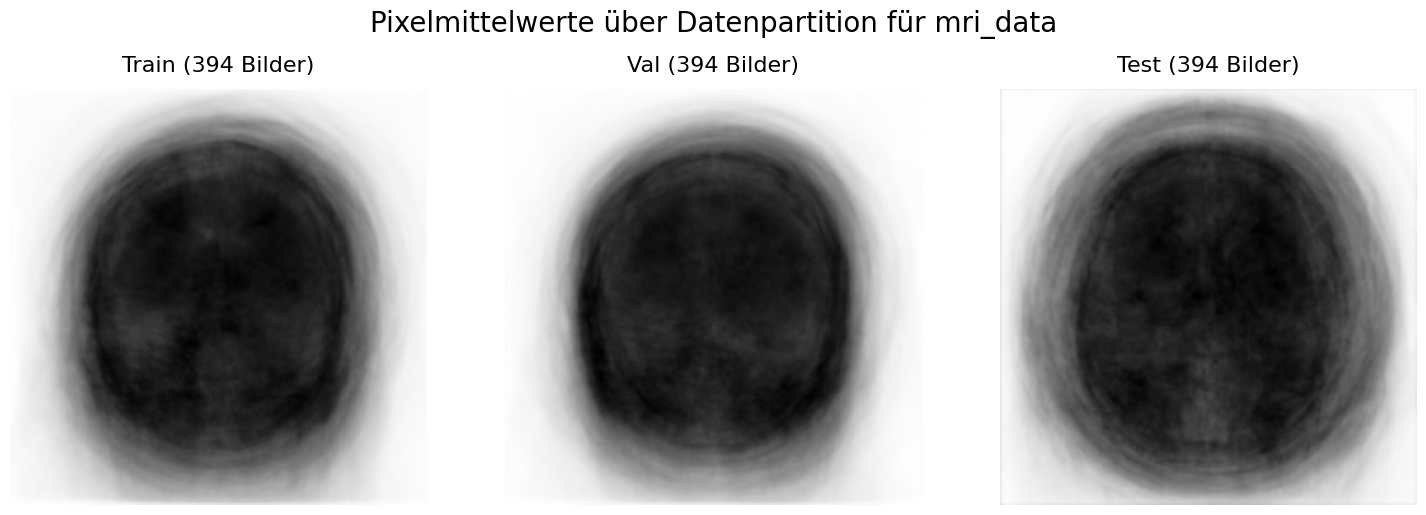
\includegraphics[width=\linewidth]{01-images/03-data/brain-pixelmittelwert-subsample-train.png}
        \caption{Visuelle Darstellung der Pixelmittelwerte einer Teilmenge von Hirntumor Bildern Datenpartition}
        \label{fig:brain-pixelmittelwert-subsample}
    \end{subfigure}
    \caption{Vergleich der Pixelmittelwerte von Hirntumor Bildern}
    \label{fig:brain-pixelmittelwert-comparison}
\end{figure}

Abbildung \ref{fig:brain-pixelmittelwert-full} zeigt die Pixelmittelwerte für alle Partitionen des Hirntumor-Datensatzes. In allen drei Partitionen ist ein dunkler Kreis erkennbar. Feine Gehirnstrukturen sind in der Validierungs- und Testpartition sichtbar, wobei sie in der Testpartition deutlicher hervortreten. Die Testpartition weist zudem mehr dunklere Pixelmittelwerte ausserhalb des Kreises auf als die anderen Partitionen. Diese Unterschiede deuten auch hier darauf hin, dass die Testpartition möglicherweise aus einer anderen Verteilung stammen als die Trainings- und Validierungspartition. Der Vergleich zwischen den Pixelmittelwertbildern aller Bilder und denen der kleineren Teilmenge von 394 Bildern pro Partition zeigt keinen grossen Unterschied.

\paragraph{Differenzbilder} \label{chap:brain-differenzenbilder}
Für die Hirntumor-Daten werden Differenzbilder analog zum Vorgehen in Kapitel \ref{chap:COVID19-differenzbilder} erstellt. Die resultierende Heatmap ist in Abbildung \ref{fig:brain-differenzenbilder} dargestellt, wobei die grundlegende Struktur der Heatmaps beibehalten wird. Als Basis für die Berechnung der Differenzen dienen die Pixelmittelwerte aus Abbildung \ref{fig:brain-pixelmittelwert-full}.

\begin{figure}[H]
    \centering
    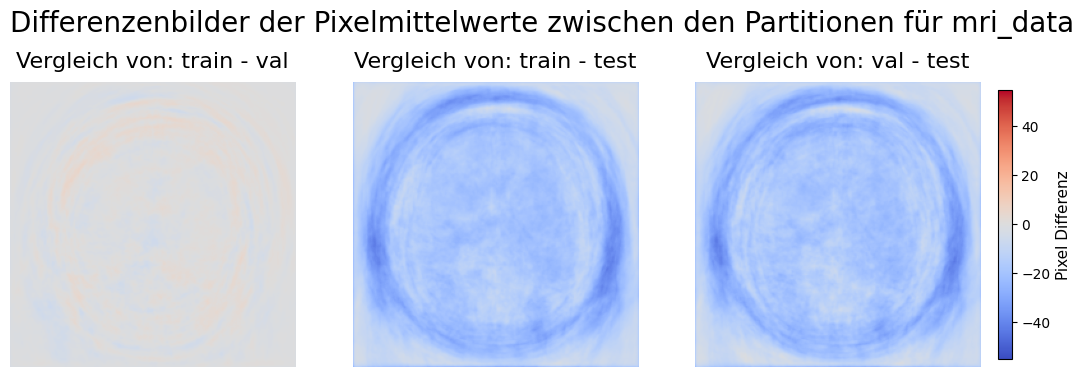
\includegraphics[width=\linewidth]{01-images/03-data/brain-differenzenbilder.png}
    \caption{Differenzbilder von jeder Datenpartition aus Abbildung \ref{fig:brain-pixelmittelwert-full}}
    \label{fig:brain-differenzenbilder}
\end{figure}

Der linke Abschnitt verdeutlicht, dass die Differenzen der durchschnittlichen Pixelwerte zwischen der Trainings- und Validierungspartition im Vergleich zu den anderen Differenzbildern minimal ausfallen. Diese geringe Abweichung lässt sich vermutlich darauf zurückführen, dass sowohl die Validierungs- als auch die Trainingspartition aus derselben ursprünglichen Datenpartition stammen.

Der mittlere und der rechte Abschnitt verdeutlichen, dass die Testpartition eine starke Abweichung zu den Trainings- und Validierungspartition aufweist. Letztere zeigen im Durchschnitt tiefere  Werte als die Testdaten, was zu negativen Differenzwerten führt und folglich ein blaues Muster in den Visualisierungen erzeugt. Dies stimmt mit den Observationen aus Kapitel \ref{chap:Differenzenbilder-TestProblemEda2-mri} überein. 

\newpage